\documentclass{article}
\usepackage{amsmath,amssymb,amsfonts}
\usepackage{pdfpages}
\usepackage{graphicx}
\usepackage{datetime}
\usepackage{braket}
\usepackage{textcomp}
\usepackage[T1]{fontenc}
\usepackage{url}
\usepackage{xcolor}
\usepackage[utf8]{inputenc}
\usepackage[english]{babel}
\usepackage[hidelinks,colorlinks=true,linkcolor=blue,citecolor=blue]{hyperref}
\usepackage{csquotes}
\usepackage[
backend=biber,
style=numeric,
sorting=none
]{biblatex}
\addbibresource{references.bib}
\pagestyle{plain}

\begin{document}
\title{\Huge \textbf{Unveiling the Uncertainty Principle: Exploring Its True Meaning and Diverse Applications}}

\author{Riddhiman Bhattacharya}
\date{January 3, 2023}
\maketitle

\begin{abstract}
The Uncertainty Principle is a fundamental concept in quantum mechanics that fundamentally affects our understanding of physical phenomena. This paper delves into the real meaning and significance of the Uncertainty Principle, shedding light on its implications across various scientific fields.
\end{abstract}

\section{Introduction}

Music provides a compelling illustration to enhance our understanding of the uncertainty principle. To determine the precise pitch of a vibrating guitar string, one must observe its oscillations over a sufficient duration to measure the length of each period. However, if we attempt to capture the exact moment of measurement, defining the precise time becomes challenging. Consequently, the specific timing of the measurement and the precise pitch become mutually exclusive. In non-technical terms, this can be expressed as follows:

\begin{equation}
\Delta f \Delta t \geq {1} 
\label{1}
\end{equation}
i.e. (error in frequency)$\times$(time taken to measure frequency) is greater than $\frac{1}{2\pi}$\cite{Heisenbergs,Musicians}.

\large
\subsection*{Heisenberg’s Uncertainty Principle in Quantum Mechanics}
 

In Quantum Mechanics, the energy of a photon is given by the equation $E = hf$, where $h$ represents Planck's constant. By multiplying equation \eqref{1} with $h$ on both sides, we obtain Heisenberg's uncertainty principle for energy:

\begin{equation}
\Delta E \Delta t \geq \frac{h}{4\pi} 
\end{equation}

Likewise, the momentum of a photon can be expressed as $\frac{h}{\lambda}$, where $\lambda$ represents the wavelength of the photon. Consequently, Heisenberg's uncertainty principle for momentum can be formulated as:

\begin{equation}
\Delta p \Delta x \geq \frac{h}{4\pi} 
\end{equation}

The above equation reveals that the position and momentum of a particle cannot be precisely measured with unlimited precision simultaneously. For instance, let's consider an electron in a hydrogen atom. It is impossible to precisely determine the position of the electron at a distance of $r$ from the nucleus because doing so would yield a momentum of zero, contradicting the concept of zero-point energy.

It is important to note that this relationship is not limited to the limitations of the measuring instrument; rather, it emerges from the inherent wave-like properties of particles, which are inherent in nature.


\section{Geometrical Derivation of HUP}
Let us consider a wave function given by state $\phi$ as:
\begin{equation}
\ket{\phi}=(\hat{x}+i\lambda\hat{p})\ket{\psi}  
\end{equation}
where $\hat{x}$, $\hat{p}$, $\lambda$ and $\ket{\psi}$ are position operator, momentum operator, arbitrary real number and arbitrary state respectively. For any $\lambda$ and $\ket{\psi}$ we have $\braket{\phi|\phi}\geq 0$. 

Therefore:
\begin{equation}
\braket{\phi|\phi}=\braket{\psi|\hat{x}^2|\psi}-i\lambda\braket{\psi|\hat{p}\hat{x}|\psi}+i\lambda\braket{\psi|\hat{x}\hat{p}|\psi}+\lambda^2\braket{\hat{p}^2}\geq 0 
\end{equation}

\begin{equation}
=\braket{\hat{p}^2}\lambda^2+\braket{i[\hat{x},\hat{p}]}\lambda+\braket{\hat{x}^2}\geq 0    
\end{equation}
The above equation can be written as:
\begin{equation}
\Delta p^2 \lambda^2 + \braket{i[\hat{x},\hat{p}]}\lambda + \Delta x^2 \geq 0    
\end{equation}
where $\Delta p$ and $\Delta x$ are the uncertainties in measuring $\hat{p}$ and $\hat{x}$ respectively. Equation 7 is similar to equation of parabola given as:

\begin{equation}
f(\lambda)=a\lambda^2 + b\lambda+c    
\end{equation}
The minimum value is at $\lambda_{min}=\frac{-b}{2a}$ which is $f(\lambda_{min})=c-\frac{b^2}{4a}$. Given $f(\lambda_{min}) \geq 0$, we obtain $ac\geq\frac{b^2}{4}$
Therefore:
\begin{equation}
\Delta x^2 \Delta p^2 \geq \frac{\braket{i[\hat{x},\hat{p}]}^2}{4}     
\end{equation}
The commutator relation of position and momentum is defined as: 
\begin{equation}
[\hat{x},\hat{p}]=i\hbar    
\end{equation}
where $\hbar$ is $\frac{h}{2\pi}$. Taking square root on both sides:
\begin{equation}
\Delta x \Delta p \geq \frac{\hbar}{2}    
\end{equation}

\subsection*{Generalized Uncertainty Principle}

The above derivation is for position and momentum operators. However, it can be generalized for any two observables(a,b), which can be shown as\cite{mmoore}:
\begin{equation}
\Delta a^2 \Delta b^2 \geq \frac{\braket{i[\hat{a},\hat{b}]}^2}{4}      
\end{equation}
i.e.
\begin{equation}
\Delta a \Delta b \geq \frac{|\braket{[\hat{a},\hat{b}]}|}{2}      
\end{equation}

\section{Quantum Squeezed Light}

The Uncertainty Principle extends beyond particles such as atoms and electrons and also applies to light waves. Light can be conceptualized as a wave composed of oscillating electric and magnetic fields, possessing both amplitude and phase. Similar to the inherent uncertainty in the position and momentum of an electron, there exists a degree of uncertainty in the amplitude and phase of a light wave.

\subsubsection*{Uncertainty Principle in Electric field}
The electric field in terms of quadrature can be given as\cite{phdthesis_eric}:
\begin{equation}
\boxed{
E(t)=\sqrt{\frac{4\pi \hbar \omega_0}{Ac}}[a_1(t)\cos{\omega_0 t}+a_2(t)\sin{\omega_0 t}]
}
\end{equation}

where a$_1$(t) and a$_2$(t) are Amplitude and Phase Quadrature respectively. The relation between these two operators is given as:
\begin{equation}
\boxed{
\Delta a_{1}^2 \Delta a_{2}^2 \geq |\frac{1}{2i}\braket{[a_1,a_2]}|^2=\frac{1}{4} } 
\label{RBTF}
\end{equation}

\textbf{Quantum squeezing} is a technique in which one of the variables of the Uncertainty principle is 'squeezed' to reduce the noise in the observation, at the expense of increased noise in the conjugate variable.

\section{Uncertainty Principle and Gravitational Waves}

\textbf{Gravitational waves} (GW) are disturbances in the fabric of space-time, typically caused by massive objects such as colliding binary black holes, supernovae, or neutron stars.

To detect these gravitational waves, \textbf{Laser Interferometer \\Gravitational-Wave Observatories} (LIGO) are utilized. These observatories have the remarkable capability of measuring length variations on the order of $10^{-21}$m. However, the primary challenge in these detectors arises from shot noise, which originates from the random fluctuations of photons in a high-power laser, as described by \cite{Chu}. As the light photons pass through these fluctuations, they experience small jostling movements, causing the light beams to shift slightly out of phase. This can be compared to a fleet of small boats navigating through a turbulent sea, where it becomes difficult to keep them together. The random phase shifts induced by shot noise can lead to the generation of false gravitational wave signals.
 


\subsection*{Squeezing at LIGO}

In order to enhance the shot-noise limit, researchers employ a technique called Quantum Squeezed Light. This technique addresses the noise in both amplitude and phase, which are the two variables governed by the Uncertainty Principle. By introducing phase-squeezed laser light into the interferometer, as described in equation \eqref{RBTF}, the noise in phase is reduced. However, this reduction in phase noise comes at the cost of an increase in amplitude noise, as illustrated in Figure 1. It is worth noting that this method has successfully improved the sensitivity of the interferometer by 25$\%$ according to the study referenced \cite{6988398}.


\begin{figure}[h]
\centering
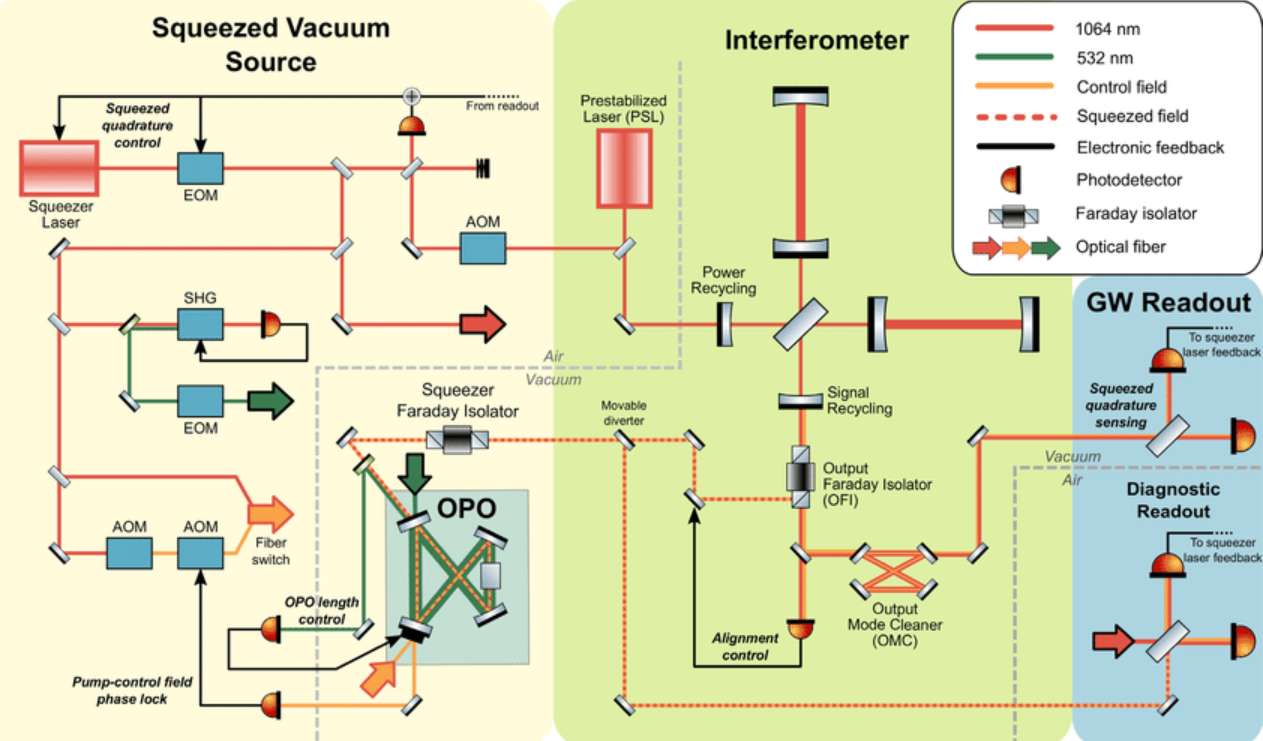
\includegraphics[scale=0.2]{LIGO.png}
\caption{\small Conceptual layout of the squeezed vacuum subsystem for Advanced LIGO. Source: \url{https://www.researchgate.net/publication/337781863_Quantum-Enhanced_Advanced_LIGO_Detectors_in_the_Era_of_Gravitational-Wave_Astronomy}}
\label{fig}
\end{figure}



\section{Conclusion}

The HUP stands as one of the most renowned concepts in physics. However, it faced staunch opposition from Albert Einstein, who believed that it didn't accurately reflect the nature of reality. Consequently, Einstein engaged in years-long debates with Werner Heisenberg and other scientists. Despite Einstein's reservations, the uncertainty principle remains integral to understanding numerous phenomena that elude explanation within the realm of classical physics. Heisenberg's elegant proposition offers insights into the prevention of atomic implosion, the mechanisms behind the sun's ability to emit light, and the revelation that the seemingly empty vacuum of space is anything but. 


\section{References}
\printbibliography[heading=none]



\end{document}